\section{Optimal Control of Pitch and Travel with Feedback (LQ)}\label{sec:prob3}
This problem involves implementing an LQ controller for optimal control with feedback. We calculated a gain matrix K using the built in MATLAB function dlqr, which solves the  discrete algebraic riccati equation. We also implemented feedback on the helicopter, and discussed if MPC is a good alternative to LQR.

\subsection{Calculating the gain matrix K}
Feedback for the system is introduced by using $u_k=u_k^*-K^T(x_k-x_k^*)$. Here $x^*$ is the optimal trajectory and $u^*$ is the optimal input sequence. A good choice for K can be found by minimizing the objective function:
\begin{equation}
J = \sum_{i=0}^\infty {\Delta x_{i+1}^TQ\Delta x_{i+1} + u_{i}^TRu_{i}}
\end{equation}
Here, Q and R are user defined diagonal matrices chosen to weight deviations in states separately. The tuning of these matrices are discussed in the next section. The built in MATLAB function dlqr is used to solve the riccati equation for the corresponding optimization problem and to compute the gain matrix K. 

\subsection{Implementing feedback on the helicopter}
The block diagram structure of the helicopter with feedback can be seen in figure (\ref{fig:day3_mdl}).
%Figure of simulink model with feedback
\begin{figure}[htb]
	\centering
   	 \makebox[\textwidth][c]{\includegraphics[width=1.2\textwidth]{figures/day3/day3_mdl}}
	\caption{Simulink model with feedback}
	\label{fig:day3_mdl}
\end{figure}

By keeping R constant at unity weight and tuning Q, we saw that by weighting travel more than pitch (50 1 1 1), the helicopter followed the travel trajectory closer than when weighting all states the same. Weighting deviation in pitch more than travel (1 1 10 1) gave a bad result. Figure (\ref{fig:day3_plot_allQ}) shows how the trajectory based on these different weights turned out compared to the mathematical optimal path. The reason for this was that the optimal pitch reference trajectory was based on a linearized model.
%HER MÅ VI HA ET SAMMENLIGNINGSPLOT MELLOM 1 1 1 1, 1 1 10 1 og 50 1 1 1 istedenfor de to under
%Figure of helicopter response for Q_LQR = diag[50 1 1 1]
\begin{figure}[htb]
	\centering
    	\makebox[\textwidth][c]{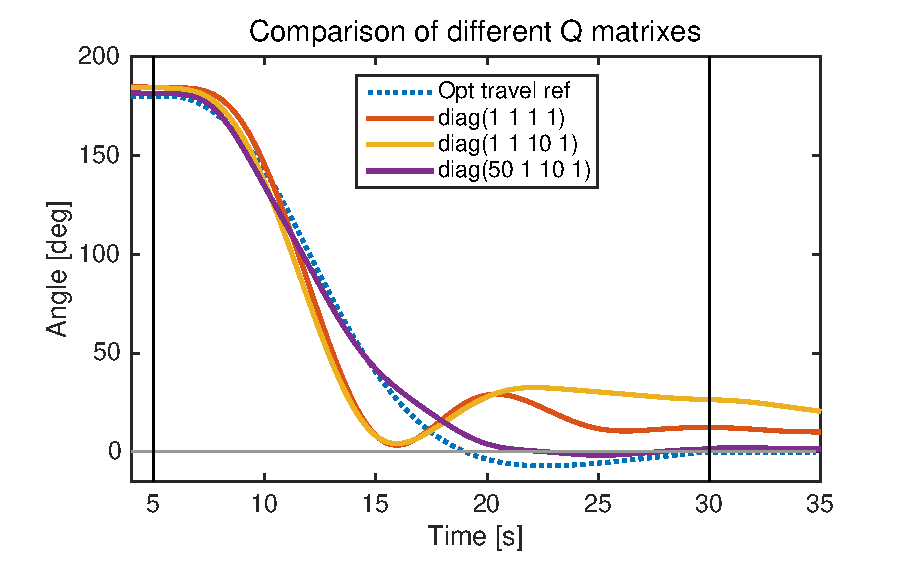
\includegraphics[width=1.2\textwidth]{figures/day3/plot_day3_allQ}}
	\caption{Plot of day 3 with differently tuned Q}
	\label{fig:day3_allQ}
\end{figure}




\subsection{Comparison between LQR and MPC}
The way to implement an MPC controller would be to calculate a new optimal trajectory at each time step. The first time step of each calculated optimal input sequence should then be used as the input $u_t$ for that time step.

The advantages of using MPC instead of LQR is that it gives the possibility to have constraints in the regulator. MPC might also result in a trajectory demanding less input, and provides implicit feedback. As we have already observed, feedback is a necessity for the control of a system with modelling errors and disturbances. 
The main disadvantage of using MPC is that the heavy calculations of finding an optimal trajectory would have to be processed during run time, hence it might not be able to control a system as fast as a helicopter.
The control hierarchy with MPC would have replaced the Advanced control layer by the Optimization layer, leading to one less layer in the hierarchy.
